\scanpage{6}
% Drawings and formula blocks follow their positions in the supplied scan.
% Formula writing at the foot is upside down in the supplied scan.
\figure{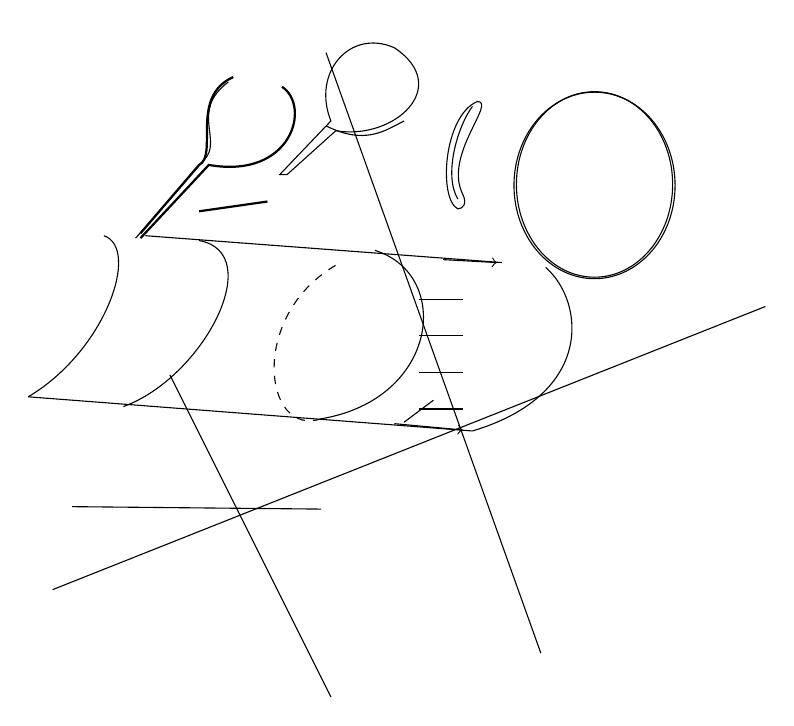
\begin{tikzpicture}[x=.62cm,y=.62cm]
\draw[thick] (1.2,3.5)--(2.4,4.9) .. controls (2.8,5.1) and (2.2,6.3) .. (3.1,6.7);
\draw[thick] (1.2,3.4)--(2.6,4.9) .. controls (4.3,4.6) and (4.7,6.1) .. (4.1,6.5);
\draw (1.1,3.4)--(2.5,5) .. controls (2.9,5.4) and (2.2,6) .. (3,6.6);
\draw[thick] (2.4,3.95)--(3.8,4.15);
\draw (4.05,4.7)--(5.1,5.8) .. controls (4.7,6.8) and (5.5,7.7) .. (6.4,7.3)
 .. controls (7.6,6.5) and (6.4,5.4) .. (5.2,5.6)--(4.2,4.7)--cycle;
\draw (5.0,5.7) .. controls (5.8,5.3) and (6.2,5.6) .. (6.6,5.8);
\draw (7.7,4.0) .. controls (7.3,4.2) and (7.4,5.9) .. (8.1,6.2)
 .. controls (8.5,6.2) and (7.4,5.1) .. (7.8,4.3) .. controls (7.9,4.1) and (7.8,4) .. (7.7,4);
\draw (7.7,4.2) .. controls (7.4,4.7) and (7.7,5.7) .. (8.0,6.1);
\draw (10.5,4.5) ellipse (1.6 and 1.9);
\draw (10.5,4.48) ellipse (1.65 and 1.91);
\draw (1.3,3.45)--(8.6,2.9) (-1.1,.15)--(8.0,-.55);
\draw (-1.1,.15) .. controls (.5,1.1) and (1.2,3.2) .. (.45,3.45);
\draw (.85,-.05) .. controls (2.5,.55) and (3.8,3.1) .. (2.4,3.35);
\draw (4.9,-.3) .. controls (7.3,.1) and (7.6,2.65) .. (6.0,3.15);
\draw[dashed] (4.9,-.3) .. controls (3.7,-.7) and (3.4,1.9) .. (5.3,2.9);
\draw (8,-.55) .. controls (10.5,.2) and (10.3,2.1) .. (9.5,2.8);
\foreach \y in {-.1,.65,1.4,2.15} {\draw (6.9,\y)--(7.8,\y);}
\draw[->] (7.4,2.96)--(8.5,2.9);
\draw[->] (6.4,-.4)--(7.8,-.53);
\draw (6.6,-.37)--(7.2,.08);
\draw (-.2,-2.1)--(4.9,-2.15);
\draw (-.6,-3.8)--(14,2.0);
\draw (5.0,7.2)--(9.4,-5.1) (1.8,.6)--(5.1,-6.0);
\end{tikzpicture}}

\[
\widetilde K_i\qquad
\unsure{\Sigma|\sum}(X_i,\partial X_i)=|\widetilde K_i|
\]

\margin{\[
|x'|,|y'|\leq\sqrt{x'^2+y'^2}\leq|x'|+|y'|
\]
\[
\int|x'|,\int|y'|\leq\int\unsure{-}\leq\int|x'|+\int|y'|
\]}

\figure{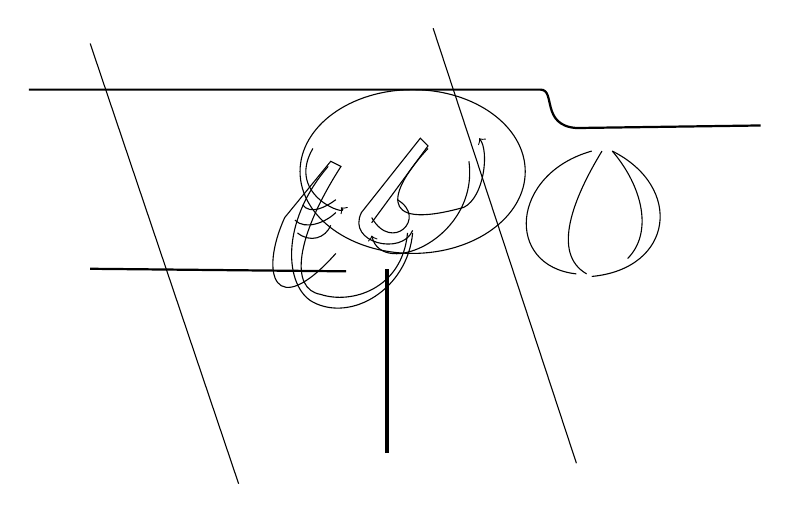
\begin{tikzpicture}[x=.65cm,y=.65cm]
\draw[thick] (-4,3.3)--(6,3.3) .. controls (6.3,3.3) and (6,2.6) .. (6.7,2.55)--(10.3,2.6);
\draw[thick] (-2.8,-.2)--(2.2,-.25);
\draw[very thick] (3,-3.8)--(3,-.2);
\draw (3.5,1.7) ellipse (2.2 and 1.6);
\draw[->] (1.55,2.15) .. controls (1,1.2) and (2.3,.8) .. (2.1,1.0);
\draw[->] (4.6,1.9) .. controls (4.8,.4) and (2.9,-.4) .. (2.7,.45);
\draw (2,.1) .. controls (.8,-1.25) and (.5,-.3) .. (1.0,.8)--(1.9,1.9)--(2.1,1.8)
 .. controls (1.2,.4) and (1.1,-.6) .. (1.7,-.7)
 .. controls (2.3,-.9) and (3.3,-.6) .. (3.4,.5);
\draw (1.85,1.8) .. controls (.9,.7) and (1.0,-.55) .. (1.55,-.85)
 .. controls (2.3,-1.25) and (3.4,-.6) .. (3.5,.5);
\draw (2.7,.7)--(3.8,2.2)--(3.65,2.35)--(2.5,.9)
 .. controls (2.2,.3) and (3.3,.05) .. (3.5,.55);
\draw[->] (3.8,2.15) .. controls (3.1,1.4) and (2.7,.5) .. (4.5,1.0)
 .. controls (4.9,1.2) and (5,2.1) .. (4.8,2.35);
\draw (2.7,.8) .. controls (3.1,.1) and (3.8,.8) .. (3.2,1.15);
\draw (1.25,.5) .. controls (1.5,.3) and (1.8,.4) .. (1.9,.65);
\draw (1.2,.75) .. controls (1.4,.55) and (1.8,.7) .. (2,.9);
\draw (1.35,1.05) .. controls (1.5,.85) and (1.8,1) .. (2.0,1.15);
\draw (7,2.1) .. controls (5.4,1.65) and (5.3,-.15) .. (6.7,-.3);
\draw (7.2,2.1) .. controls (6.65,1.2) and (6.2,.1) .. (6.9,-.3);
\draw (7.4,2.1) .. controls (8.8,1.4) and (8.6,-.2) .. (7,-.35);
\draw (7.4,2.1) .. controls (8,1.4) and (8.2,.5) .. (7.7,.0);
\draw (-2.8,4.2)--(.1,-4.4) (3.9,4.5)--(6.7,-4.0);
\end{tikzpicture}}

\[
\widetilde K=\varinjlim_{x\in K\setminus L}K_x,
\qquad K_x=\{y\in K\mid y\leq x\}
\]
\[
\left\{\begin{array}{l}
|\widetilde K|-|\widetilde L|\xrightarrow{\sim}|K|-|L|\\
(\widetilde K,\widetilde L)\text{ est ``pur''}
\end{array}\right.
\]

\diagram{\begin{tikzcd}[column sep=large,row sep=large]
\widetilde K \arrow[r,"\pi"] & K\ {\deleted{\unsure{\cup}}}\\
\widetilde L=\pi^{-1}(L) \arrow[u,phantom,"\cup",description] \arrow[r] & L \arrow[u,bend right=55]
\end{tikzcd}}

\deleted{$\widetilde L_0=\pi^{-1}(L_0)\subset\widetilde K_0$}

\deleted{$\widetilde L=T$}
% archive foliation: 5
